\documentclass[12pt, twoside]{article}
\usepackage[francais]{babel}
\usepackage[T1]{fontenc}
\usepackage[latin1]{inputenc}
\usepackage[left=5mm, right=5mm, top=3mm, bottom=3mm]{geometry}
\usepackage{float}
\usepackage{graphicx}
\usepackage{array}
\usepackage{multirow}
\usepackage{amsmath,amssymb,mathrsfs}
\usepackage{soul}
\usepackage{textcomp}
\usepackage{eurosym}
 \usepackage{variations}
\usepackage{tabvar}


\pagestyle{empty}

\begin{document}

 
\begin{flushleft}
NOM PRENOM: \ldots \ldots \ldots \ldots \ldots \ldots \ldots \ldots \ldots
 

\end{flushleft} 
 
 \medskip
 
\begin{center}
{\fbox{$4^{e}3$ \qquad \qquad \textbf{\Large{Devoir surveill� 5 }}
\qquad \qquad 17/03/2011}}
\end{center}

\enskip


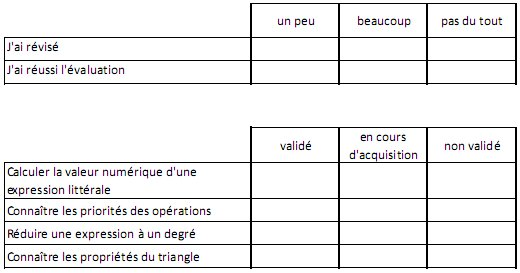
\includegraphics[width=14cm]{images/socle.jpg}


\bigskip

\bigskip


\ul{\textbf{Exercice 1}}: \textit{(3 points)}

R�duire si possible les expressions suivantes (vous
marquerez ``pas possible'' si vous pensez qu'on ne peut pas r�duire).


\begin{center}
\begin{tabular}{ccc}
\begin{minipage}{6cm}
$A=9x+5x$ \ldots \ldots \ldots \ldots

$B=0 \times a$ \ldots \ldots \ldots \ldots
\end{minipage}
&
\begin{minipage}{6cm}
$C=2b \times 3b$ \ldots \ldots \ldots \ldots

$D=5+2y$ \ldots \ldots \ldots \ldots
\end{minipage}
&
\begin{minipage}{6cm}
$E=t+5t^2$ \ldots \ldots \ldots \ldots

$F=-4u \times 5$ \ldots \ldots \ldots \ldots
\end{minipage}
\end{tabular}
\end{center}

\bigskip


\ul{\textbf{Exercice 2}}: \textit{(2,5 points)}

Pour chaque question, cocher la ou les bonnes
r�ponses (il peut y avoir une ou plusieurs r�ponses par ligne).

\begin{center}
\begin{tabular}{|c|c|c|c|c|}
\hline
\quad & \begin{minipage}{3cm}
        L'expression est factoris�e
    
        \end{minipage} & 

\begin{minipage}{3cm}
L'expression est
d�velopp�e
        \end{minipage}
 & 

\begin{minipage}{3cm}
L'expression est r�duite 
        \end{minipage}
& 

\begin{minipage}{3cm}
L'expression est quelconque
        \end{minipage} \\

\hline
 \quad $A=(2y+3)(-4+y)$ \quad & \quad & \quad & \quad & \\
 

\hline

\quad $B=2(3+t)-4$ \quad &  \quad & \quad & \quad & \\

\hline

\quad $C=9u-7u+4$ \quad &  \quad & \quad & \quad & \\

\hline

 \quad $D=4x^2+3x-7$ \quad &  \quad & \quad & \quad & \\   


\hline 
\end{tabular}
\end{center}

\bigskip


\ul{\textbf{Exercice 3}}: \textit{(2,5 points)} \quad Un calcul non d�taill� 
donnera 0 point.

\begin{enumerate}
  \item Calculer la valeur de l'expression $G=4z-5$ pour $z=-3$.
  
  \ldots \ldots \ldots \ldots \ldots \ldots \ldots \ldots \ldots \ldots \ldots
  \ldots \ldots \ldots \ldots \ldots \ldots \ldots \ldots \ldots \ldots \ldots
  \ldots \ldots \ldots \ldots \ldots \ldots \ldots \ldots \ldots \ldots \ldots
  \ldots \ldots 
  
   \ldots \ldots \ldots \ldots \ldots \ldots \ldots \ldots \ldots \ldots \ldots
  \ldots \ldots \ldots \ldots \ldots \ldots \ldots \ldots \ldots \ldots \ldots
  \ldots \ldots \ldots \ldots \ldots \ldots \ldots \ldots \ldots \ldots \ldots
  \ldots \ldots   
  
   \ldots \ldots \ldots \ldots \ldots \ldots \ldots \ldots \ldots \ldots \ldots
  \ldots \ldots \ldots \ldots \ldots \ldots \ldots \ldots \ldots \ldots \ldots
  \ldots \ldots \ldots \ldots \ldots \ldots \ldots \ldots \ldots \ldots \ldots
  \ldots \ldots     
  
  \item Calculer la valeur de l'expression $H=2x^2+3x-5$ pour $x=5$.
  
   \ldots \ldots \ldots \ldots \ldots \ldots \ldots \ldots \ldots \ldots \ldots
  \ldots \ldots \ldots \ldots \ldots \ldots \ldots \ldots \ldots \ldots \ldots
  \ldots \ldots \ldots \ldots \ldots \ldots \ldots \ldots \ldots \ldots \ldots
  \ldots \ldots
  
      \ldots \ldots \ldots \ldots \ldots \ldots \ldots \ldots \ldots \ldots \ldots
  \ldots \ldots \ldots \ldots \ldots \ldots \ldots \ldots \ldots \ldots \ldots
  \ldots \ldots \ldots \ldots \ldots \ldots \ldots \ldots \ldots \ldots \ldots
  \ldots \ldots           
  
        
  
   \ldots \ldots \ldots \ldots \ldots \ldots \ldots \ldots \ldots \ldots \ldots
  \ldots \ldots \ldots \ldots \ldots \ldots \ldots \ldots \ldots \ldots \ldots
  \ldots \ldots \ldots \ldots \ldots \ldots \ldots \ldots \ldots \ldots \ldots
  \ldots \ldots   
\end{enumerate}


\bigskip


\ul{\textbf{Exercice 4}}: \textit{(4 points)}

D�velopper les expressions suivantes et les r�duire.

\begin{tabular}{cc}
$U=(x-2)(3+4x)$ \qquad \qquad \qquad \quad & \qquad \qquad  \qquad \qquad
\qquad \quad $V=3(y-4)+(2y+1)(5+y)$
\\

\bigskip

\quad & \quad \\
\quad & \quad \\
\quad & \quad \\
\quad & \quad \\
\quad & \quad \\
\quad & \quad \\

\quad & \quad \\
\quad & \quad \\
\quad & \quad \\
\quad & \quad \\

\end{tabular}







\bigskip


\ul{\textbf{Exercice 5}}: \textit{(5 points)}

Trois soeurs se partagent un forfait familial de t�l�phone de 480 minutes par
mois.

Emilie t�l�phone t minutes.

Zo� t�l�phone 10 minutes de moins qu'Emilie.

Yasmine t�l�phone 2 fois plus que Zo�.


\begin{enumerate}
  \item Ecrire en fonction de t le nombre de minutes t�l�phon�es par chacune
  des soeurs.
  \item Ecrire en fonction de t le nombre total de minutes t�l�phon�es pour les
  trois soeurs. R�duire l'expression trouv�e.
  \item Ecrire en fonction de t le nombre de minutes restant � t�l�phoner
  (c'est-�-dire ce qu'il reste du forfait).
  \item  Emilie a t�l�phon� 120 minutes. Calculer le temps de
  forfait restant.
\end{enumerate}


   \ldots \ldots \ldots \ldots \ldots \ldots \ldots \ldots \ldots \ldots \ldots
  \ldots \ldots \ldots \ldots \ldots \ldots \ldots \ldots \ldots \ldots \ldots
  \ldots \ldots \ldots \ldots \ldots \ldots \ldots \ldots \ldots \ldots \ldots
  \ldots \ldots 
  
   \ldots \ldots \ldots \ldots \ldots \ldots \ldots \ldots \ldots \ldots \ldots
  \ldots \ldots \ldots \ldots \ldots \ldots \ldots \ldots \ldots \ldots \ldots
  \ldots \ldots \ldots \ldots \ldots \ldots \ldots \ldots \ldots \ldots \ldots
  \ldots \ldots 
  
 \ldots \ldots \ldots \ldots \ldots \ldots \ldots \ldots \ldots \ldots \ldots
  \ldots \ldots \ldots \ldots \ldots \ldots \ldots \ldots \ldots \ldots \ldots
  \ldots \ldots \ldots \ldots \ldots \ldots \ldots \ldots \ldots \ldots \ldots
  \ldots \ldots 
  
   \ldots \ldots \ldots \ldots \ldots \ldots \ldots \ldots \ldots \ldots \ldots
  \ldots \ldots \ldots \ldots \ldots \ldots \ldots \ldots \ldots \ldots \ldots
  \ldots \ldots \ldots \ldots \ldots \ldots \ldots \ldots \ldots \ldots \ldots
  \ldots \ldots 
  
   \ldots \ldots \ldots \ldots \ldots \ldots \ldots \ldots \ldots \ldots \ldots
  \ldots \ldots \ldots \ldots \ldots \ldots \ldots \ldots \ldots \ldots \ldots
  \ldots \ldots \ldots \ldots \ldots \ldots \ldots \ldots \ldots \ldots \ldots
  \ldots \ldots 
  
   \ldots \ldots \ldots \ldots \ldots \ldots \ldots \ldots \ldots \ldots \ldots
  \ldots \ldots \ldots \ldots \ldots \ldots \ldots \ldots \ldots \ldots \ldots
  \ldots \ldots \ldots \ldots \ldots \ldots \ldots \ldots \ldots \ldots \ldots
  \ldots \ldots 
  
   \ldots \ldots \ldots \ldots \ldots \ldots \ldots \ldots \ldots \ldots \ldots
  \ldots \ldots \ldots \ldots \ldots \ldots \ldots \ldots \ldots \ldots \ldots
  \ldots \ldots \ldots \ldots \ldots \ldots \ldots \ldots \ldots \ldots \ldots
  \ldots \ldots 
  
   \ldots \ldots \ldots \ldots \ldots \ldots \ldots \ldots \ldots \ldots \ldots
  \ldots \ldots \ldots \ldots \ldots \ldots \ldots \ldots \ldots \ldots \ldots
  \ldots \ldots \ldots \ldots \ldots \ldots \ldots \ldots \ldots \ldots \ldots
  \ldots \ldots 
  
  
   \ldots \ldots \ldots \ldots \ldots \ldots \ldots \ldots \ldots \ldots \ldots
  \ldots \ldots \ldots \ldots \ldots \ldots \ldots \ldots \ldots \ldots \ldots
  \ldots \ldots \ldots \ldots \ldots \ldots \ldots \ldots \ldots \ldots \ldots
  \ldots \ldots 
  
  
  
  
\bigskip


\ul{Exercice 6}: \textit{(3 points)}

\begin{tabular}{cc}
\begin{minipage}{11cm}
\begin{enumerate}
  \item D�montrer que ABC est un triangle rectangle en C.
  \item Calculer CD. Justifier votre r�ponse.
 
 
\end{enumerate}
\end{minipage}
&
\begin{minipage}{7cm}
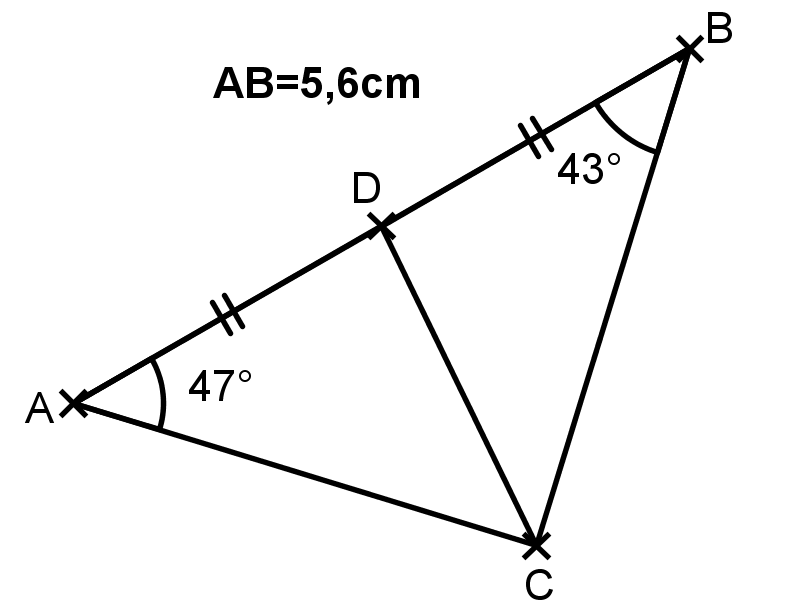
\includegraphics[width=55mm]{images/ex6.png}  
\end{minipage}
\end{tabular}

\enskip

   \ldots \ldots \ldots \ldots \ldots \ldots \ldots \ldots \ldots \ldots \ldots
  \ldots \ldots \ldots \ldots \ldots \ldots \ldots \ldots \ldots \ldots \ldots
  \ldots \ldots \ldots \ldots \ldots \ldots \ldots \ldots \ldots \ldots \ldots
  \ldots \ldots 
  
  
   \ldots \ldots \ldots \ldots \ldots \ldots \ldots \ldots \ldots \ldots \ldots
  \ldots \ldots \ldots \ldots \ldots \ldots \ldots \ldots \ldots \ldots \ldots
  \ldots \ldots \ldots \ldots \ldots \ldots \ldots \ldots \ldots \ldots \ldots
  \ldots \ldots 
  
   \ldots \ldots \ldots \ldots \ldots \ldots \ldots \ldots \ldots \ldots \ldots
  \ldots \ldots \ldots \ldots \ldots \ldots \ldots \ldots \ldots \ldots \ldots
  \ldots \ldots \ldots \ldots \ldots \ldots \ldots \ldots \ldots \ldots \ldots
  \ldots \ldots 
  
  
   \ldots \ldots \ldots \ldots \ldots \ldots \ldots \ldots \ldots \ldots \ldots
  \ldots \ldots \ldots \ldots \ldots \ldots \ldots \ldots \ldots \ldots \ldots
  \ldots \ldots \ldots \ldots \ldots \ldots \ldots \ldots \ldots \ldots \ldots
  \ldots \ldots 
  
  
   \ldots \ldots \ldots \ldots \ldots \ldots \ldots \ldots \ldots \ldots \ldots
  \ldots \ldots \ldots \ldots \ldots \ldots \ldots \ldots \ldots \ldots \ldots
  \ldots \ldots \ldots \ldots \ldots \ldots \ldots \ldots \ldots \ldots \ldots
  \ldots \ldots
  
     \ldots \ldots \ldots \ldots \ldots \ldots \ldots \ldots \ldots \ldots \ldots
  \ldots \ldots \ldots \ldots \ldots \ldots \ldots \ldots \ldots \ldots \ldots
  \ldots \ldots \ldots \ldots \ldots \ldots \ldots \ldots \ldots \ldots \ldots
  \ldots \ldots 
  
  
   \ldots \ldots \ldots \ldots \ldots \ldots \ldots \ldots \ldots \ldots \ldots
  \ldots \ldots \ldots \ldots \ldots \ldots \ldots \ldots \ldots \ldots \ldots
  \ldots \ldots \ldots \ldots \ldots \ldots \ldots \ldots \ldots \ldots \ldots
  \ldots \ldots 
  
  
   \ldots \ldots \ldots \ldots \ldots \ldots \ldots \ldots \ldots \ldots \ldots
  \ldots \ldots \ldots \ldots \ldots \ldots \ldots \ldots \ldots \ldots \ldots
  \ldots \ldots \ldots \ldots \ldots \ldots \ldots \ldots \ldots \ldots \ldots
  \ldots \ldots  
  
     \ldots \ldots \ldots \ldots \ldots \ldots \ldots \ldots \ldots \ldots \ldots
  \ldots \ldots \ldots \ldots \ldots \ldots \ldots \ldots \ldots \ldots \ldots
  \ldots \ldots \ldots \ldots \ldots \ldots \ldots \ldots \ldots \ldots \ldots
  \ldots \ldots 
  
 
\end{document}
